\documentclass[letterpaper,11pt]{article}
%--------------Document configuration begins--------------
\usepackage{fullpage}
\usepackage[numbers]{natbib} 	%\citet{jon90} --> Jones et al. [21], \citep{jon90} --> [21]
\usepackage[colorlinks]{hyperref}
%--------------Document configuration ends--------------

\usepackage{microtype}

\usepackage{commandsrm}
\usepackage{commands_theo} 			%Theorems, lemmas, proofs, etc
%Load cleveref last
\usepackage[capitalize]{cleveref}


\bibliographystyle{plain}

\title{\vspace{-1cm} \bf Approximate DP and Regret Analysis   \vspace{-1.3cm}}
\author{}
\begin{document}
\maketitle

\section{Probing}

\paragraph{Problem Statement}
At each time $t$, an arrival is drawn from a set of $n$ types, such that $j\in[n]$ arrives with probability $p_j$.
An arrival can be \emph{active or inactive} with a known probability; inactive arrivals generate no reward, but do consume resources.
A type $j$ has an associated reward $r_j\geq 0$ and a probability $q_j\in [0,1]$: Conditioned on being of type $j$, the reward of an arrival is $r_j\cdot \Ber(q_j)$.
The decision-maker is given hiring and probing budgets $B_h,B_p\in\N$.
If he chooses to probe an arrival, then he can see the realization of the Bernoulli before accepting, thus protecting him against inactive arrivals.
He can also choose to accept the arrival without probing, in such case the reward is random, but it does not consume probing budget.

Even with full knowledge of the arrivals $Z_j$, the problem of adaptively choosing which arrivals to probe or accept is difficult.
Indeed, the state space has size $\prod_jZ_j = \Omega(\T^n)$.
This is the reason why the prevalent focus in recent research has been to bound the adaptivity gap first and then search for simpler policies \cite{adaptivity_gaps}.

We define \off to be the agent who knows the arrival process $Z(t)$, but does not know the result of the Bernoulli trials.
The value function $\voff(t,b_h,b_p)$ is determined by the natural Bellman Equations.
We start by providing an upper bound to the value function, defined by the following decision variables representing total numbers, not binary values: $y_j$ is the number of type $j$ we probed, $x_{ja}$ is the number of type $j$ accepted without probing and $x_{jp}$ is the number of type $j$ accepted after probing.

\begin{proposition}\label[proposition]{prop:probing_relaxation}
For any $b_h,b_p\in\N$, $t\in[\T]$ and realization $Z$ of arrivals, $\voff(t,b_h,b_p)$ is upper bounded by
\begin{equation}\label{eq:probing_relaxation}
\begin{array}{rrll}
(P^\star)\quad \max  & \sum_jr_j(x_{jp}+q_jx_{ja}) \\
\text{s.t.}& \sum_j y_j & \leq b_p \\
& \sum_j(x_{jp}+x_{ja}) &\leq b_h \\
&  x_{ja} + y_j & \leq Z_j(t)  &\forall j\in [n] \\
& x_{jp} &\leq q_jy_j & \forall j \in [n] \\
& y_j,x_{j,a},x_{j,p}&\geq 0 & \forall j\in[n].
\end{array}
\end{equation}
\end{proposition}	
\begin{proof}
Consider any policy for \off which determines when to probe, accept or reject.
The policy induces a random trajectory, which is determined by the realization of the Bernoulli variables, not the arrivals, since the later are given.
Define the following random variables, counting the number of times in which a type $j$: was probed, denoted $Y_j$; was accepted without probing, $X_{ja}$; and was accepted after probing, $X_{jp}$.
Finally, let $Y_{j}^+,X_{ja}^+$ be the number of active from among those probed or accepted, respectively.
We assume w.l.o.g.\ that, among the probed elements, \off takes only active ones.

Our aim is to argue that, replacing the aforementioned r.v.\ with their expectations, yields a feasible solution to $(P^\star)$.
It holds $\voff(t,b_h,b_p) = \E[\sum_j r_j(X_{jp}+X_{ja}^+)]$ and $\E[X_{ja}^+|X_{ja}]=q_jX_{ja}$, thus
\[
\voff(t,b_h,b_p) = \sum_jr_j(\E[X_{jp}]+q_j\E[X_{ja}]).
\] 

With the exception of the constraint $x_{jp}\leq q_jy_j$, $X_{ja},Y_j,X_{jp}$ satisfy a.s.\ all the constraints of $(P^\star)$, hence their expectations do too.
Observe that $X_{jp}\leq Y_{j}^+$ and $\E[Y_j^+]=q_j\E[Y_j]$, thus $\E[X_{jp}]\leq q_j\E[Y_j]$.
To summarize, $\voff(t,b_h,b_p)$ equals the value of the feasible solution given by the expectations, so $v(P^\star)$ can be only larger.
\end{proof}

\section{Probing II: Beyond Bernoulli and formulation as a MCDP}

\paragraph{Problem Statement}
Same as before, but now a type $j$ is associated with values $r_{j1},r_{j2}>0$ and $q_{j1},q_{j2}\in[0,1]$ such that $q_{j1}+q_{j2}\leq 1$.
The reward of a type $j$ is $r_{jk}$ with probability $q_{jk}$, $k\in\crl{1,2}$, and $0$ with probability $q_{j0}\defeq1-q_{j1}-q_{j2}$.
There is a conceptual gap from this case with three values and the binary (active/inactive), but the extension from three to multiple values is straightforward.
We denote $\bar r_j\defeq r_{j1}q_{j1}+r_{j2}q_{j2}$.

Let us define an \emph{input process} indexed by $t\in[2T]$.
At even times, the input reveals the type $j$ and at odd times it reveals the actual realization given probabilities $q_{jk}$.
Formally, let $(\xit)$ be a Markov chain in the state space $[n]\cup\crl{(j,k):j\in[n],k=0,1,2}$.
The transition probabilities are given by $P_{j,(j,k)}=q_{jk}$, $P_{(j,k),j'}=p_{j'}$.
For $\xi^{2t-1}=(j,k)$ we define $r(\xi^{2t-1})=r_{jk}$.

The state space for our problem can be described as $\St=\crl{(b_h,b_p),(b_h,b_p,\diamond):b_h,b_p\in\N,\diamond\in \crl{\texttt{a,p,r}}}$, see \cref{fig:probing_states}.
The component $\diamond$ indicates if we are in the accept, probe or reject stage.
There is never a $\diamond$ at times $2t$ and, at $2t-1$, feasible controls are different for distinct $\diamond$.

\begin{figure}
\centering
\scalebox{0.9}{%
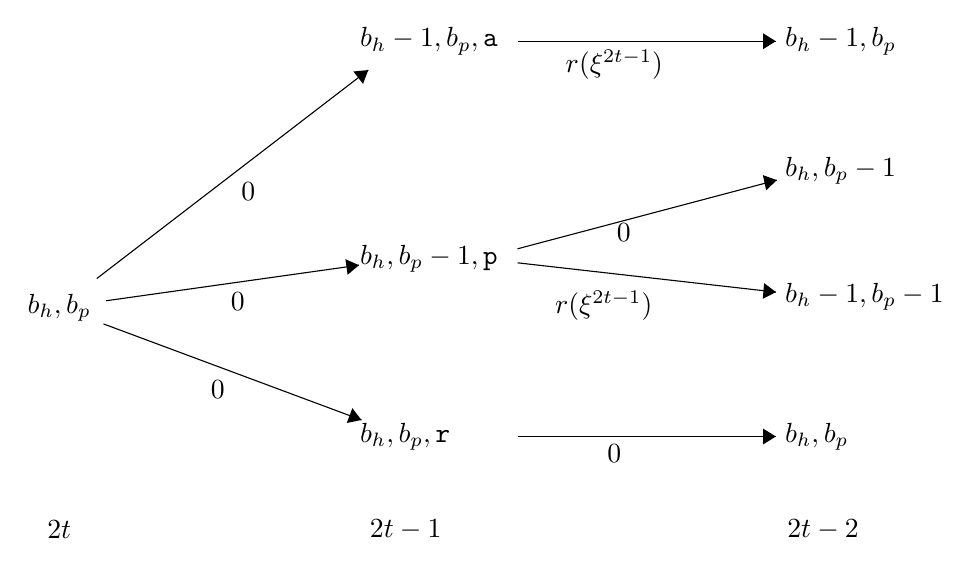
\begin{tikzpicture}[scale=0.2]
\tikzstyle{every node}+=[inner sep=0pt]

\draw (5.9,-25.9) node {$b_h,b_p$};

\draw (5.9,-40) node {$2t$};
\draw (27.9,-40) node {$2t-1$};
\draw (54.4,-40) node {$2t-2$};

\draw (30,-9) node[text width=2cm] {$b_h-1,b_p,\texttt{a}$};
\draw (30,-22.8) node[text width=2cm] {$b_h,b_p-1,\texttt{p}$};
\draw (30,-34.1) node[text width=2cm] {$b_h,b_p,\texttt{r}$};

\draw (57,-9) node[text width=2cm] {$b_h-1,b_p$};
\draw (57,-17.2) node[text width=2cm] {$b_h,b_p-1$};
\draw (57,-34.1) node[text width=2cm] {$b_h,b_p$};
\draw (57,-25.2) node[text width=2cm] {$b_h-1,b_p-1$};


\draw [black] (8.28,-24.07) -- (25.52,-10.83);
\fill [black] (25.52,-10.83) -- (24.58,-10.92) -- (25.19,-11.71);
\draw (17.91,-17.95) node [below] {$0$};
\draw [black] (8.87,-25.48) -- (24.93,-23.22);
\fill [black] (24.93,-23.22) -- (24.07,-22.84) -- (24.21,-23.83);
\draw (17.24,-24.94) node [below] {$0$};
\draw [black] (8.71,-26.95) -- (25.09,-33.05);
\fill [black] (25.09,-33.05) -- (24.51,-32.3) -- (24.16,-33.24);
\draw (15.97,-30.52) node [below] {$0$};

\draw [black] (35,-9) -- (51.4,-9);
\fill [black] (51.4,-9) -- (50.6,-8.5) -- (50.6,-9.5);
\draw (41.15,-9.5) node [below] {$r(\xi^{2t-1})$};
\draw [black] (35,-22.18) -- (51.46,-17.82);
\fill [black] (51.46,-17.82) -- (50.58,-17.5) -- (50.79,-18.47);
\draw (41.75,-20.58) node [below] {$0$};
\draw [black] (35,-23.07) -- (51.41,-24.93);
\fill [black] (51.41,-24.93) -- (50.66,-24.36) -- (50.57,-25.36);
\draw (40.47,-24.83) node [below] {$r(\xi^{2t-1})$};
\draw [black] (35,-34.1) -- (51.4,-34.1);
\fill [black] (51.4,-34.1) -- (50.6,-33.6) -- (50.6,-34.6);
\draw (41.15,-34.6) node [below] {$0$};
\end{tikzpicture}
}
\caption{Transitions for the online probing problem. 
Numbers below the arrows represent the reward of a transition.
At time $2t$ the possible actions are: accept, probe and reject.
At $2t-1$, depending on $\diamond$, we can either accept or reject and $b_h$ may be discounted.
}
\label{fig:probing_states}
\end{figure}

The natural relaxation is similar to \cref{eq:probing_relaxation}, but it presents a new challenge.
For binary cases, it was obvious that, if \off wants to probe an arrival, he will always accept it if it is active.
In this case it could be that \off probes $j$ in hope of observing $r_{j2}$ and will reject $r_{j1}$.
We must, therefore, reason about \off's actions at all times, instead of just at even times as before and concluding with structural properties.

Let $\calX\defeq\Rp^{4n}$ be the space for the decision variables.
Note that, by definition, $Z_j(2t-1)=Z_j(2t)-\In{\xi^{2t}=j}$.
In \cref{eq:probing_even,eq:probing_odd} we present two similar functions, observe that they differ by the last two constraints only.

\begin{equation}\label{eq:probing_even}
\begin{array}{rrll}
\varphi(2t,b,Z,\xi^{2t}) \; \max & \multicolumn{3}{l}{\sum_{j,k}r_{jk}(x_{(j,k)a}+q_{jk}x_{ja})} \\
\text{s.t.}& \sum_j x_{jp} & \leq b_p \\
& \sum_{j,k}x_{(j,k)a}+\sum_jx_{ja} &\leq b_h \\
&  x_{ja} +x_{jp} & \leq Z_j(t)  & j\in [n] \\
& x_{(j,k)a} &\leq q_{jk}x_{jp} &  j \in [n],k\in [2].
\end{array}
\end{equation}
\begin{equation}\label{eq:probing_odd}
\begin{array}{rrll}
\varphi(2t-1,b,Z,\xi^{2t-1}) \; \max & \multicolumn{3}{l}{\sum_{j,k}r_{jk}(x_{(j,k)a}+q_{jk}x_{ja})} \\
\text{s.t.}& \sum_j x_{jp} & \leq b_p \\
& \sum_{j,k}x_{(j,k)a}+\sum_jx_{ja} &\leq b_h \\
&  x_{ja} + x_{jp} & \leq Z_j(t)-\In{\xi^{2t}=j}  & j\in [n] \\
& x_{(j,k)a} &\leq q_{jk}x_{jp} + \In{\xi^{2t-1}=(j,k)}&  j \in [n],k\in [2].
\end{array}
\end{equation}

An argument as in \cref{prop:probing_relaxation} shows that $\voff(t,b)\leq \varphi(t,b,Z,\xit)$.
We can pretend, thus, that \off agrees to receive rewards according to $\varphi$.
To make this precise, we need a map between two worlds, since \onl decides on actions \texttt{a,p,r} and \off on points in $\calX$.

\begin{lemma}
Let $\bar X\in\calX$ be a maximizer of $\varphi(2t,b,Z,\xi^{2t})$.
Say $\xi^{2t}=j$, then, at time $2t$, \off is satisfied with the following actions:
\begin{enumerate}
\item Accept if $\bar X_{ja}\geq 1$
\item Probe if $\bar X_{jp}\geq 1$
\item Reject if $\bar X_{ja}+\bar X_{jp}\leq Z_j(t)-1$
\end{enumerate}
At time $2t-1$, \off is satisfied accepting type $(j,k)$ in a probing stage if $\bar X_{jp}\geq 1$ and $\bar X_{(j,k)a}\geq 1$.
\end{lemma}
\begin{proof}
\off is satisfied solving the following problem, where the actions correspond, respectively, to accept, probe and reject
\[
\max\crl{\bar r_j+\E_{\xi^{2t-2}}[\varphi(2t-2,b-e_h,Z,\xi^{2t-2})], \E_{\xi^{2t-2}}[\varphi(2t-1,b-e_p,Z,\xi^{2t-1})], \E_{\xi^{2t-2}}[\varphi(2t-2,b,Z,\xi^{2t-2})]}.
\]
For the accept and reject options the expectation is redundant, since all the necessary information to solve the problem is given in $Z$.
This is not true for the probe option, since \off is unaware of $\xi^{2t-2}$.
By Jensen's inequality, $\E_{\xi^{2t-2}}[\varphi(2t-1,b-e_p,Z,\xi^{2t-1})]\leq \varphi(2t-1,b-e_p,Z,\E[\xi^{2t-1}])$, where we are abusing notation to denote that in \cref{eq:probing_odd} we are replacing $\In{\xi^{2t-1}=(j,k)}$ by $q_{jk}$.
It follows now that \off is also satisfied solving the problem 
\[
\max\crl{\bar r_j+\varphi(2t-2,b-e_h,Z,\xi^{2t-2}), \varphi(2t-1,b-e_p,Z,\E[\xi^{2t-1}])], \varphi(2t-2,b,Z,\xi^{2t-2})}.
\]
Finally, we can relate each of these options with the optimum of $\varphi(2t,b,Z,\xi^{2t})$ in the cases (1), (2) and (3).
The argument at odd times $2t-1$ is similar. 
\end{proof}


\section{General Version}

Consider a DP with state space $\St$ and a sequence of inputs $\xit\in\Xi$ for $t\in[\T]$, where $t$ is the \emph{time to-go}.
We assume $\xit$ evolves as a Markov chain on state space $\Xi$, with known transition matrix and initial distribution.

For every state $s\in\St$, arrival $\xi$ and control $u\in\U$, we  collect a reward $\Re(s,\xi,u)$, which could be $-\infty$, and transition to the state $\Tr(s,\xi,u)$.
Observe that the reward function is deterministic, but the input $\xi$ is random, thus making the reward itself at each time a random variable.
We stress that, at each time $t$, the decision-maker first observes $\xit$ and based on that makes a decision.
\anote{
The only difference is that in MCDP the reward depends on a pair of states (current and transition), but I think that would be redundant.
}
Any time dependence will be embedded in the process $\xit$, e.g., if the randomness represents unknown demand, the state of the Markov chain could be of the form $\J=\crl{(t,x):t\in[\T],x\in\Rp}$, where the first component gives us the time and the second the demand for the period.
This formulation is known as a Markov Chance-Decision Process \cite[chap 13]{online_book}.


Given this formulation, the value function at any given time can be expressed as
\begin{equation}
v(t,s) = \E_{\xit,\ldots,\xi^1}\brk*{\max_{u^t,\ldots,u^1}\sum_{\tau=1}^t\Re(S^\tau,\xi^\tau,u^\tau) \text{ s.t. }  S^t=s \text{ and } S^{\tau-1}=\Tr(S^\tau,\xi^\tau,u^\tau) \forall \tau<t }.
\end{equation}

Even if we reveal the entire input sequence, the problem inside of the expectation could be NP-Hard.
This yields another motivation for online algorithms: by pretending the input arrives online, it gives a way of efficiently approximating a hard problem.

We can define \off as the agent that knows the entire sequence, but this is too pessimistic and in general does not lead to sensible algorithms.
Instead, we will define a hierarchy of such agents, each with more information.

We now start imposing assumptions to guarantee two things: (1) we can find a \emph{tractable relaxation} to the maximization problem and (2) the relaxation is useful for \onl.
The first point will be achieved by obtaining a concave maximization program with convex constraints, while the second requires \emph{revealing some, but not all, information} to \off.

\paragraph{Assumption: Finite Dimension}
We identify $\St\subseteq \R^\ds$ and $\U\subseteq\R^\du$.

\paragraph{Assumption: Linear Transitions}
There are operators $A,B$ such that, given a control $u^{t+1}$ at state $S^{t+1}$, the system transitions as follows
\[
S^{t} = AS^{t+1} + Bu^{t+1}, t\in[\T-1], \quad 
S^T \text{ given}.
\]
By a simple induction, given a sequence of controls $u^\tau$ for $\tau=\T,\ldots,t+1$, the state at time $t$ is
\[
S^t = A^{T-t}S^T + \sum_{\tau=t+1}^\T A^{\tau-1-t}Bu^\tau, \quad t\in[T].
\]

If $A$ is idempotent (a projection), then the formula simplifies greatly.
\anote{	For now we will assume $A$ is the identity, but the projection thing is important. The results shouldn't change.}
In this case we have the simpler formula
\begin{equation}\label{eq:linear_state}
S^t = S^T + \sum_{\tau=t+1}^\T Bu^\tau, \quad t\in[T].
\end{equation}

For notation simplicity, we assume $0\in \R^\du$ is always a valid action.
\anote{I'm not sure how restrictive this is.}

\paragraph{Assumption: Subadditve Concave Rewards}
The reward function $\Re(s,\xi,u)$ depends on $s,\xi$ only to specify feasible controls, i.e., combinations of arrivals and controls that give reward $-\infty$.
Formally, define $\U(s,\xi)\defeq \crl{u\in\U: \Re(s,\xi,u)>-\infty}$.
We assume that $\Re(s,\xi,u)$ is just a function of $u$ provided that $u\in\U(s,\xi)$.

Additionally, we assume that either (1) $\Re(u)$ is concave and subadditive or (2) there is a concave function $\tilde \Re:\U^\T\to\R$ such that $\sum_t\Re(u^t)\leq \tilde \Re(\sum_t u^t)$.

The operator $B$ is also subadditive.

\anote{In principle $\Re$ is defined only for discrete points, so we actually require an extension that takes real numbers.}

\paragraph{Assumption: Indexing for controls and states}
The hope is that we can aggregate arrivals in a convenient way.
For this aim, we need to reduce the information in $\Xi$.
We assume there is a mapping $J:\Xi\to[n]$.
Intuitively, if $\xi,\xi'\in\J$ are such that $J(\xi)=J(\xi')$, then they are identical in terms of reward and feasibility constraints.
As a shortcut, we use $\Jt\defeq J(\xit)$.

Similarly, there is a mapping $I:\St\to [m]$ and we denote $\It=I(S^t)$.
We assume there is a convex function $f:\R^\ds\times\R^\du\to\R^d$, called \emph{feasibility function}, and discrete sets $\U_{ij}$ such that
\[
\U(s,\xi) = \crl{u\in \U_{I(s),J(\xi)}: f(s,u)\geq 0}.
\]

We denote $d_{ij}\defeq \abs{U_{ij}}$ the number of available controls and enumerate its elements as $\U_{ij} = \crl{u_{ijk}: k\in [d_{ij}]}$. 
We define the processes $Z_j(t)\defeq\sum_{\tau\leq t}\In{J^\tau=j}=\sum_{\tau\leq t}\In{J(\xi^\tau)=j}$ and $Z_{ij}(t) \defeq \sum_{\tau\leq t}\In{J^\tau=j,I^\tau=i}$.

\anote{For now I'm thinking of a discrete set of controls (e.g. accept, reject) and the results will depend on the number of controls.
Nevertheless, I think there is an extension to, e.g., reject or sell $k$ units, with $k\in\N$.
It is important that the ``basis" has small dimension, rather than the controls themselves. 
}

\paragraph{Assumption: Monotonicity}
The state $S^t$ is monotone over time.
Additionally, the feasibility function $f(s,u)$ are also monotone in $s$.
\anote{This is not fundamental in the following sense: the state can be monotone by intervals, e.g., the inventory descreases in $T,\ldots,T/2$, but at $T/2$ we can restock, then it decreases again in $T/2-1,\ldots,1$.
}

Now we will separate the processes into \emph{revealed information} and its counterpart, the \emph{concealed information}.
\off will have access to the revealed information, but only distributional information for the rest.
We denote by $\Theta\subseteq [n]$ the set of indexes we reveal, meaning that \off knows $Z_j(\T)$ for $j\in\Theta$.
Below we present the natural fluid relaxation of the concealed information, which we call \emph{the canonical relaxation}.
The first set of constraints, those involving $Z_{ij}$, are referred to as \emph{dynamics equations}.
The constraints defined by $f$ are, naturally, called \emph{feasibility equations}.

\begin{definition}[Canonical Relaxation]
If $\Theta$ are the revealed processes, and we denote $Z_\Theta(T)$ as a vector with the components $j\in\Theta$, then the following is called the canonical relaxation given $\Theta$
\begin{equation}\label{eq:theta_relaxation}
\begin{array}{rrll}
(P_\Theta)\quad \max  & \tilde \Re\prn*{\sum_{i\in [m]}\sum_{k\in [k_i]}x_{k,i}u_{k,i}} \\
\text{s.t.}&  \sum_k x_{ijk} & \leq \E[Z_{ij}(T)| Z_\Theta(T) ]  &\forall i\in[m], j\in[n] \\
& f\prn*{S^\T+B\sum_{i,j,k}u_{ijk}x_{ijk},0}&\geq 0  \\
& x_{ijk}&\geq 0 & \forall i\in [m], j\in [n], k\in [d_{ij}] .
\end{array}
\end{equation}
\end{definition}

\begin{proposition}
For any choice of indexes $\Theta$, $v(T,S^T)\leq v(P_\Theta)$	
\end{proposition}

\begin{definition}[Valid Relaxation]
	TODO
\end{definition}


\bibliography{biblio}

\end{document}
